%% Do not edit unless you really know what you are doing.
\documentclass[12pt,a4paper]{report}
\usepackage[T1]{fontenc}
\usepackage[latin1]{inputenc}
\usepackage{color,geometry,graphicx}
\usepackage[absolute]{textpos}
\usepackage{pdfpages}
\usepackage{float,textcomp,amsmath,paralist,calc}
\usepackage{natbib}
\usepackage{xr}
\usepackage[titletoc]{appendix}
\geometry{verbose,a4paper,tmargin=1in,bmargin=1in,lmargin=1in,rmargin=1in}
\newcommand{\ap}{\textquotesingle}
\newcommand{\sq}[1]{\textquotesingle{#1}\textquotesingle}
\setlength\parindent{0pt}

\definecolor{gray}{rgb}{0.8,0.8,0.8}

\newcommand{\frontmatter}{\cleardoublepage
  \pagenumbering{roman}}
\newcommand{\mainmatter}{\cleardoublepage
  \pagenumbering{arabic}}
\newcommand{\backmatter}{\cleardoublepage}

%%%%%%%%%%%%%%%%%%%%%%%%%%%%%% User specified LaTeX commands.
%\renewcommand{\baselinestretch}{1.5}

% hyperlinks to sections and references
%\usepackage[pdftex,bookmarks=true,bookmarksnumbered=true,pdfpagemode=None,pdfstartview=FitH,pdfpagelayout=SinglePage,pdfborder={0 0 0}]{hyperref}
\newcommand{\tsup}[1]{\textsuperscript{#1}}
\newenvironment{desclist}[1]
{\begin{list}{}
{\renewcommand\makelabel[1]{{##1}\hfill}
\settowidth\labelwidth{\makelabel{#1}}
\setlength\leftmargin{\labelwidth+\labelsep}}}
{\end{list}}

\newenvironment{adescription}[1]
{\begin{list}{}
{\renewcommand\makelabel[1]{\texttt{##1}\hfill}
\settowidth\labelwidth{\makelabel{#1}}
\setlength\leftmargin{\labelwidth+\labelsep}}}
{\end{list}}

% Package name and version
\def\pack{SPECFEM3D\_GEOTECH}
\def\packver{\pack\ 1.2}

\begin{document}
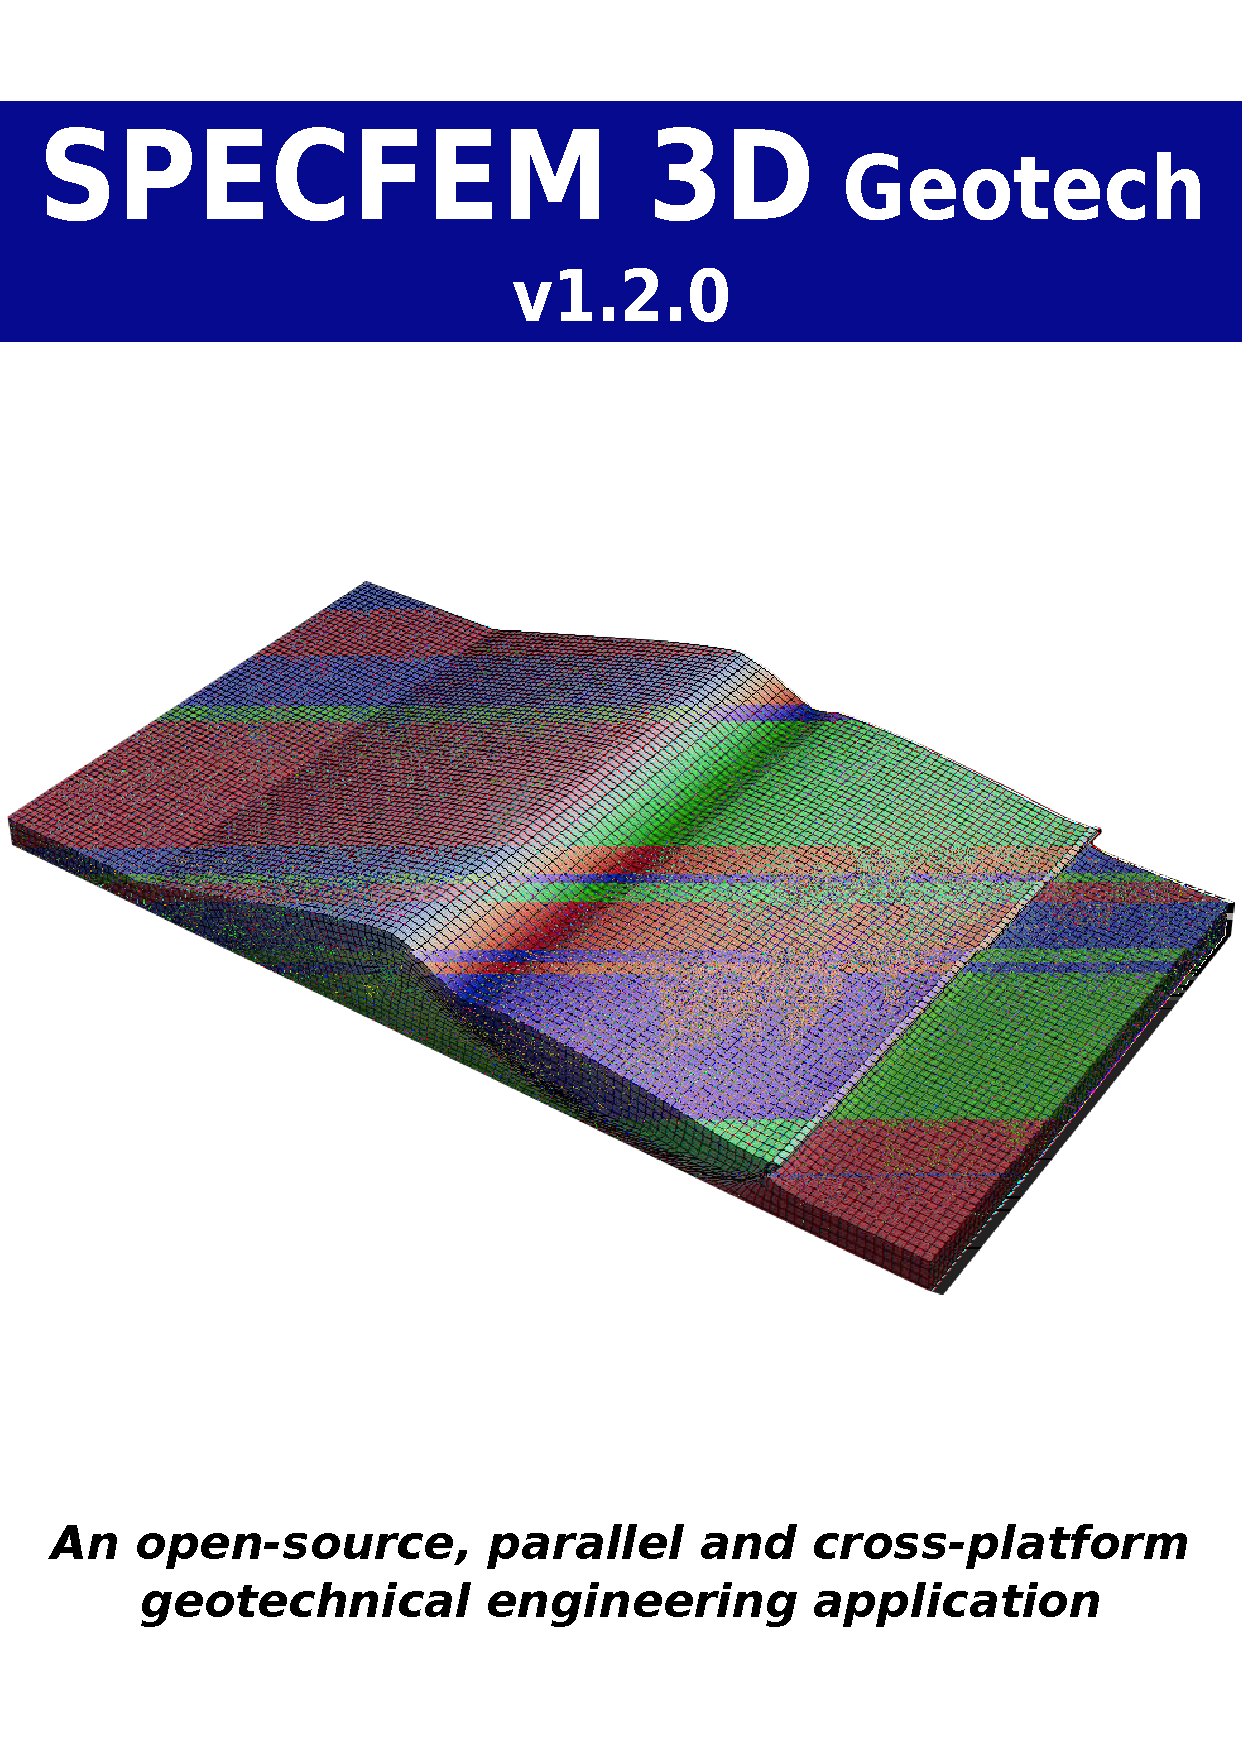
\includepdf[fitpaper]{cover}

\thispagestyle{empty} % no page number
\title{\textbf{\packver \\
User Manual}}

\author{
Hom Nath Gharti\footnote{Previously at: NORSAR, Norway}, Princeton University, USA \\
Dimitri Komatitsch, Aix-Marseille University, France\\
Volker Oye, NORSAR, Norway \\
Roland Martin, University of Toulouse, France \\
Jeroen Tromp, Princeton University, USA \\
Zhenzhen Yan, Institute of Remote Sensing and Digital Earth, CAS, China
}


\maketitle

\frontmatter

\addcontentsline{toc}{chapter}{Licensing}
\chapter*{Licensing}
%
%\packver\ \\
%Copyright 2010-2011 Hom Nath Gharti\\
%
%This file is part of \packver.\\
%
\packver\ is free software: you can redistribute it and/or modify
it under the terms of the GNU General Public License as published by
the Free Software Foundation, either version 3 of the License, or
(at your option) any later version.\\

\packver\ is distributed in the hope that it will be useful,
but WITHOUT ANY WARRANTY; without even the implied warranty of
MERCHANTABILITY or FITNESS FOR A PARTICULAR PURPOSE.  See the
GNU General Public License for more details.\\

You should have received a copy of the GNU General Public License
along with \linebreak\packver.  If not, see <\texttt{http://www.gnu.org/licenses/}>.\\

\clearpage

\addcontentsline{toc}{chapter}{Acknowledgments}
\chapter*{Acknowledgments}
This work was funded in part by the Research Council of Norway,
and supported by industry partners BP, Statoil, and Total. Some of the routines were imported and modified from the ``Programming the finite element method''~\citep{smith2004} and the original ``SPECFEM3D'' package~\citep[e.g.,][]{komatitsch1998,komatitsch1999,peter2011}.

\clearpage

\tableofcontents
\clearpage

\mainmatter
\chapter{Introduction}
\label{chap:intro}
\section{Background}

\pack\ is a free and open-source command-driven software for 3D slope stability analysis~\citep[for more details see][]{gharti2012a} and simulation of 3D multistage excavation~\citep[for more details see][]{gharti2012b} based on the spectral-element method~\citep[e.g.,][]{patera1984,canuto1988,seriani1994,faccioli1997,komatitsch1998,komatitsch1999,peter2011}. The slope stability and the excavation routines were originally started from the routines found in the book ``Programming the finite element method''~\citep{smith2004}. The software can run on a single processor as well as multi-core machines or large clusters. It is written mainly in FORTRAN 90, and parallelized using
MPI~\citep{gropp1994,pacheco1997} based on domain decomposition. For the domain decomposition, the open-source graph partitioning library SCOTCH~\citep{pellegrini1996} is used. The element-by-element preconditioned conjugate-gradient method~\citep[e.g.,][]{hughes1983,law1986,king1987,barragy1988} is implemented to solve the linear equations. For elastoplastic failure,
a Mohr-coulomb failure criterion is used with a viscoplastic strain method~ \citep{zienkiewicz1974}.\\

This program does not automatically determine the factor of safety of slope stability. Simulations can be performed for a series of safety factors. After plotting the safety factor verses maximum displacement curve, one can determine the factor of safety of the given slope. Although the software is optimized for slope stability analysis and multistage excavation, other relevant simulations of quasistatic problems in solid (geo)mechanics can also be performed with this software.\\

The software currently does not include an inbuilt mesher. Existing tools, such as Gmsh~\citep{geuzaine2009}, CUBIT/Trelis~\citep{cubit2011}, TrueGrid~\citep{truegrid2006}, etc., can be used for hexahedral meshing, and the resulting mesh file can be converted to the input files required by \pack. Output data can be visualized and processed using the open-source visualization application ParaView (\texttt{www.paraview.org}).

\section{Status summary}
\begin{desclist}{Pseudo-static earthquake loading}
\item[Serial run]        : Yes
\item[Parallel run with MPI]        : Yes
\item[Slope stability analysis]        : Yes
\item[Multistage excavation]           : Yes
\item[Gravity loading]                 : Yes
\item[Surface loading]                 : Yes (point load, uniformly distributed load, linearly distributed load) [Experimental]
\item[Water table]                     : Yes [Experimental]
\item[Pseudo-static earthquake loading]: Yes [Experimental]
\item[Automatic factor of safety]      : No
\end{desclist}

\section{Changes made since the last version}
\begin{itemize}
\item File format of the displacement boundary conditions has changed (See Section~\ref{subsec:dispbc}).
\item Now the program can be run from any locations.
\item Main routines are modularized in preparation to add other features in coming versions.
\item Removed all instances of run time warning for temporary arrays.
\item Added step-by-step tutorials for both serial and parallel runs.
\item Added GiD mesh converter.
\item Improved EXODUS mesh converter.
\item Fixed several minor bugs.
\item Structural change and overall code cleanup.
\end{itemize}

\chapter{Getting started}
\label{chap:start}
\section{Package structure}
The original \pack\ package comes in a single compressed file \linebreak\texttt{\pack.tar.gz}, which can be extracted using \texttt{tar} command:\\

\texttt{tar -zxvf \pack.tar.gz}\\

or using, for example, \texttt{7-zip (www.7-zip.org)} under WINDOWS.\\

Alternatively, the package can be obtained using Git.\\

For the latest stable release, use the following Git command:\\
\\
\texttt{git clone -{}-recursive https://github.com/geodynamics/specfem3d\_geotech.git}\\
\\
For the development version, use the following Git command:\\
\\
\texttt{git clone -{}-recursive -{}-branch devel https://github.com/geodynamics/specfem3d\_geotech.git}\\
\\
The package has the following structure:\\



\texttt{\pack/}
\begin{adescription}{~~CMakeLists.txt}
\item[~~COPYING]               : License.
\item[~~README]                : brief description of the package.
\item[~~CMakeLists.txt]        : CMake configuration file.
\item[~~bin/]                  : all object files and executables are stored in this folder.
\item[~~doc/]                  : documentation files for the \pack\ package. If built this file is created.
\item[~~input/]                : contains input files.
\item[~~partition/]            : contains partition files for parallel processing.
\item[~~output/]               : default output folder. All output files are stored in this folder unless the different output path is defined in the main input file.
\item[~~src/]                  : contains all source files.
\item[~~util/]                 : contains several utilities source files.
\end{adescription}

\section{Prerequisites}
\begin{itemize}[-]
  \item \underline{CMake build system}. The CMake version $\ge$ 2.8.4 is necessary to configure the software. It is free and open-source, and can be downloaded from \texttt{www.cmake.org}. In order to check if the CMake is already installed, type\\
  \texttt{cmake -{}-version}

  \item \underline{Make utility}. The make utility is necessary to build the software using Makefile. This utility is usually installed by default in most LINUX systems. Under WINDOWS, one can use Cygwin (\texttt{www.cygwin.com}) or MinGW (\texttt{www.mingw.org}) to install the make utility.  In order to check if the CMake is already installed, type\\
  \texttt{make -{}-version}
  \item \underline{A recent FORTRAN compiler}. The software is written mainly in FORTRAN 90, but it also uses a few FORTRAN 2003 features (e.g., streaming IO). These features are already available in most of the FORTRAN compilers, e.g., gfortran version $\ge$ 4.2 (\texttt{gcc.gnu.org/wiki/GFortran}) and g95 (\texttt{www.g95.org}).
\end{itemize}
  Following libraries are necessary for parallel processing.
\begin{itemize}[-]
  \item \underline{A recent MPI library}. It should be built with the same FORTRAN compiler used to compile the software. Please see \texttt{www.open-mpi.org} or \linebreak\texttt{www.mcs.anl.gov/research/projects/mpich2} for details on how to install MPI library and how to run MPI programs.
  \item \underline{SCOTCH graph partitioning library}. This library should be compiled with the same\linebreak FORTRAN compiler used to compile the software. Please see\linebreak \texttt{www.labri.fr/perso/pelegrin/scotch} for details on how to install SCOTCH.
\end{itemize}

  Finally, the following compiler is necessary to build the documentation (this file):
\begin{itemize}[-]
  \item \underline{\LaTeX\ compiler}. This is necessary to compile the documentation files.
\end{itemize}

\section{Configure}
\label{sec:configure}

Software package \pack\ is configured using CMake, and the package uses an out-of-source build. Hence, \underline{DO NOT} build in the same source directory. Let's say the full path to the package (source directory) is \texttt{\$HOME/source/\pack}.

\begin{itemize}
\item Create a separate build directory, e.g.,\\
\texttt{mkdir \$HOME/build/\pack}

\item Go to the build directory \\
\texttt{cd \$HOME/build/\pack}

\item CMake configuration \\
CMake has a command-line interface \texttt{cmake}, and interactive interfaces \texttt{ccmake} a curses interface and \texttt{cmake-gui} a GUI. For more options and flexibility, we recommend using either of the interactive interfaces. For example, type:\\
\\
\texttt{ccmake \$HOME/source/\pack} \\
\\
This will open the CMake GUI (Figure~\ref{fig:cmake}), in which you can select several options as described below.
\end{itemize}
You can also set the necessary compilers explicitly, and configure the package with the default options by typing, for example,\\
\\
\texttt{CC=gcc CXX=g++ FC=gfortran MPIFC=mpif90 ccmake \$HOME/source/\pack} \\
\\
for GNU compilers.\\
\\
OR\\
\\
\texttt{CC=icc CXX=icpc FC=ifort MPIFC=mpif90 ccmake \$HOME/source/\pack} \\
\\
for Intel compilers.


\begin{figure}[ht]
\centering
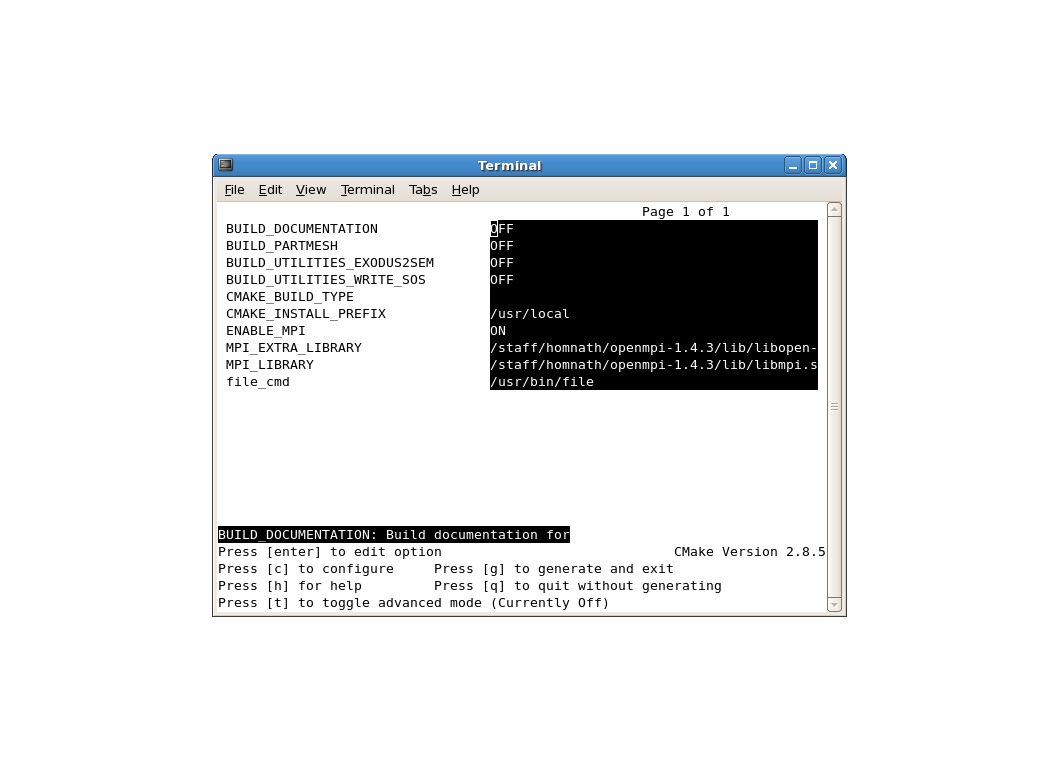
\includegraphics[scale=1.0]{cmake}
\caption{CMake configuration of \pack\ .}
\label{fig:cmake}
\end{figure}

CMake configuration is an iterative process (See Figure~\ref{fig:cmake}):
\begin{itemize}
\item Configure (\sq{c} key or \sq{Configure} button)
\item Change variables' values if necessary
\item Generate (\sq{g} key or \sq{Generate} button. This key or button appears once the configurtion is successful.)
\end{itemize}

If WARNINGS or ERRORS occur, press the \sq{e} key (or the \sq{OK} button) to return to configuration. These steps have to be repeated until successful configuration. Then, press the \sq{g} key (or the \sq{Generate} button) to generate build files. Check carefully that all necessary variables are set properly. Unless configuration is successful, \sq{g} key or \sq{Generate} button is not enabled. Sometimes, the \sq{c} key or \sq{Configure} button has to be pressed repeatedly until \sq{g} key or \sq{Generate} is enabled. Initially, all variables may not be visible. To see all variables, toggle advanced mode by pressing the \sq{t} key (or the Advanced button).
To set or change a variable, move the cursor to the variable and press \sq{Enter} key. If the variable is a boolean (ON/OFF), it will flip the value on pressing the \sq{Enter} key. If the variable is a string or a file, it can be edited. For more details, please see the CMake documentation (\texttt{www.cmake.org}).
\\

Following are the main CMake variables for the \pack\ (See Figure~\ref{fig:cmake})

\colorbox{gray}{
\parbox{15.5cm}{
\begin{adescription}{BUILD\_UTILITIES\_EXODUS2SEM}
\item[BUILD\_DOCUMENTATION]           : If \texttt{ON}, the user manual (this file) is created. The default is \texttt{OFF}.
\item[BUILD\_PARTMESH]                : If \texttt{ON}, the \texttt{partmesh} program is built. The default is \texttt{OFF}. The \texttt{partmesh} program is necessary to partition the mesh for parallel processing.
\item[BUILD\_EXODUS2SEMGEOTECH]   : If \texttt{ON}, the \texttt{exodus2semgeotech} program is built. The default is \texttt{OFF}. The \texttt{exodus2semgeotech} program convert exodus mesh file to input files required by the \pack\ package (see also Chapter~\ref{chap:util}).
\item[BUILD\_GID2SEMGEOTECH]   : If \texttt{ON}, the \texttt{gid2semgeotech} program is built. The default is \texttt{OFF}. The \texttt{gid2semgeotech} program convert GiD mesh file to input files required by the \pack\ package (see also Chapter~\ref{chap:util}).
\item[BUILD\_WRITE\_SOS]   : If \texttt{ON}, the \texttt{write\_sos} program is built. The default is \texttt{OFF}. The \texttt{write\_sos} program writes a EnSight SOS file necessary for the parallel visualization (see also Chapter~\ref{chap:util}).
\item[ENABLE\_MPI]                    : If \texttt{ON}, the main parallel program \texttt{psemgeotech} is built otherwise main serial program \texttt{semgeotech} is built. The default is \texttt{OFF}.
\item[SCOTCH\_LIBRARY\_PATH]          : This is required if \texttt{BUILD\_PARTMESH} is \texttt{ON}. If not found automatically, it can be set manually.
\item[CMAKE\_Fortran\_COMPILER]       : This defines the Fortran compiler. If not found automatically or the automatically found compiler is not correct, it can be set manually.
\item[MPI\_Fortran\_COMPILER]       : This defines the MPI Fortran compiler. This is required if \texttt{ENABLE\_MPI} is \texttt{ON}. If not found automatically or the automatically found compiler is not correct, it can be set manually.
\end{adescription}
}}\\

{\emph{Note 1: If}} \texttt{CMAKE\_Fortran\_COMPILER} {\emph{has to be changed, first change this and configure, and then change other variables if necessary and configure.}}\\
{\emph{Note 2: Even if some of the above variables are set }} \texttt{ON}{\emph{, if appropriate working compilers are not found, corresponding variables are internally set}} \texttt{OFF} {\emph{with WARNING messages.}}

\section{Compile}
\begin{itemize}[]
  \item Once configuration and generation are successful, the necessary build files are created. Now to build the main program, type: \\
  \texttt{make}

  \item On multi-processor systems (let's say eight processors), type:\\
  \texttt{make -j 8}

  \item To clean, type\\
  \texttt{make clean}
  \item{\emph{Note: If reconfiguration is necessary, it is better to delete all Cache files of the build directory.}}
\end{itemize}

\section{Run}
\subsubsection{Serial run}
\begin{itemize}[-]
\item To run the serial program, type \\
    \texttt{./bin/semgeotech} \emph{input\_file\_name}

    Example:

    \texttt{./bin/semgeotech ./input/validation1.sem}

\end{itemize}

\subsubsection{Parallel run}
\begin{itemize}[-]
\item To partition the mesh, type \\
    \texttt{./bin/partmesh} \emph{input\_file\_name}

    Example:

    \texttt{./bin/partmesh ./input/validation1.psem}

\item To run the parallel program, type \\
    \texttt{mpirun -n} \emph{number\_of\_nodes} \texttt{./bin/psemgeotech} \emph{input\_file\_name} \\

    OR

    \texttt{mpirun -n} \emph{number\_of\_nodes} \texttt{-{}-hostfile} \emph{host\_file} \texttt{./bin/psemgeotech} \emph{input\_file\_name}

    Example:

    \texttt{mpirun -n 8 ./bin/psemgeotech ./input/validation1.psem}
\end{itemize}

{\emph{Note: see Chapter~\ref{chap:input} for details on input and input files. Try to run one or more examples included in}} \texttt{input/}{\emph{. By default, example files included in the package are not copied to build directory during build process. If necessary, copy files within}} \texttt{input/} {\emph{folder of source directory to the}} \texttt{input/} {\emph{folder of build directory.}}

\chapter{Input}
\label{chap:input}
\section{Main input file}

The main input file structure is motivated by the ``E3D''~\citep{larsen1995} software package. The main input file consists of legitimate input lines defined in the specified formats. Any number of blank lines or comment lines can be placed for user friendly input structure. The blank lines contain no or only white-space characters, and the comment lines contain "\#" as the first character. \\

Each legitimate input line consists of a line type, and list of arguments and corresponding values. All argument-value pair are separated by comma (,). If necessary, any legitimate input line can be continued to next line using FORTRAN 90 continuation  character "\&" as an absolute last character of a line to be continued. Repetition of same line type is not allowed.\\

Legitimate input lines have the format\\
{\it{line\_type}} $arg_1=val_1$, $arg_2=val_2$, ......., $arg_n=val_n$\\

Example:\\
\texttt{preinfo: nproc=8, ngllx=3, nglly=3, ngllz=3, nenod=8, ngnod=8, \& \\
inp\_path=\sq{./input}, part\_path=\sq{./partition}, out\_path=\sq{./output/}}\\
\\
OR
\\
\\
\texttt{preinfo:   \quad\&\\
          \hspace*{18pt} nproc=8,\&\\
          \hspace*{18pt} ngllx=3,\&\\ 
          \hspace*{18pt} nglly=3,\&\\ 
          \hspace*{18pt} ngllz=3,\&\\ 
          \hspace*{18pt} nenod=8,\&\\ 
          \hspace*{18pt} ngnod=8,\&\\
          \hspace*{18pt} inp\_path=\sq{./input},\&\\
          \hspace*{18pt} part\_path=\sq{./partition},\&\\ 
          \hspace*{18pt} out\_path=\sq{./output/}}\\
\\
All legitimate input lines should be written in lower case. Line type and argument-value pairs must be separated by a space. Each argument-value pair must be separated by a comma(,) and a space/s. No space/s are recommended before line type and in between argument name and "=" or "=" and argument value. If argument value is a string, the FORTRAN 90 string (i.e., enclosed within single quotes) should be used, for example, \texttt{inp\_path=\sq{./input}}. If the argument value is a vector (i.e., multi-valued), a list of values separated by space (no comma!) shoud be used, e.g, \texttt{srf=1.0 1.2 1.3 1.4}.

\subsection{Line types}

Only the following line types are permitted.
\begin{adescription}{traction:}
\item[preinfo:]  preliminary information of the simulation
\item[mesh:]     mesh information
\item[bc:]      boundary conditions information
\item[traction:] traction information [optional]
\item[stress0:] initial stress information [optional]. It is generally necessary for multistage excavation.
\item[material:] material properties
\item[eqload:]   pseudo-static earthquake loading [optional]
\item[water:]    water table information [optional]
\item[control:]  control of the simulation
\item[save:]  options to save data
\end{adescription}

\subsection{Arguments}

Only the following arguments under the specified line types are permitted.\\

\texttt{\underline{preinfo:}}

\begin{adescription}{nl\_maxiter}
  \item[nproc] : number of processors to be used for the parallel processing [integer > 1]. Only required for parallel processing.
  \item[ngllx] : number of Gauss-Lobatto-Legendre (GLL) points along $x$-axis [integer > 1].
  \item[nglly] : number of GLL points along $y$-axis [integer > 1].
  \item[ngllz] : number of GLL points along $z$-axis [integer > 1]. \\\\
  {\emph{Note: Although the program can use different values of}} \texttt{ngllx}, \texttt{nglly}, {\emph{and}} \texttt{ngllz}, {\emph{it is recommended to use same number of GLL points along all axes.}}
  \item[inp\_path]  : input path where the input data are located [string, optional, default $\Rightarrow$ \texttt{\sq{./input}}].
  \item[part\_path] : partition path where the partitioned data will be or are located [string, optional, default $\Rightarrow$ \texttt{\sq{./partition}}]. Only required for parallel processing.
  \item[out\_path]  : output path where the output data will be stored [string, optional, default $\Rightarrow$ \texttt{\sq{./output}}].\\
\end{adescription}


\texttt{\underline{mesh:}}
\begin{adescription}{nl\_maxiter}
  \item[xfile] : file name of $x$-coordinates [string].
  \item[yfile] : file name of $y$-coordinates [string].
  \item[zfile] : file name of $z$-coordinates [string].
  \item[confile]: file name of mesh connectivity [string].
  \item[idfile]: file name of element IDs [string].
  \item[gfile]: file name of ghost interfaces, i.e., partition interfaces [string]. Only required for parallel processing.\\
\end{adescription}

\texttt{\underline{bc:}}
\begin{adescription}{nl\_maxiter}
  \item[uxfile]: file name of displacement boundary conditions along $x$-axis [string].
  \item[uyfile]: file name of displacement boundary conditions along $y$-axis [string].
  \item[uzfile]: file name of displacement boundary conditions along $z$-axis [string].\\
\end{adescription}

\texttt{\underline{traction:}}
\begin{adescription}{nl\_maxiter}
  \item[trfile]: file name of traction specification [string].\\
\end{adescription}

\texttt{\underline{stress0:}}
\begin{adescription}{nl\_maxiter}
  \item[type]: type of initial stress [integer, optional, 0 = compute using SEM itself, 1 = compute using simple vertical lithostatic relation, default $\Rightarrow$ 0].
  \item[z0]: datum (free surface) coordinate [real, m]. Only required if \texttt{type}=1.
  \item[s0]: datum (free surface) vertical stress [real, kN/m\tsup{2}]. Only required if \texttt{type}=1.
  \item[k0]: lateral earth pressure coefficient [real].
  \\
\end{adescription}

\texttt{\underline{material:}}
\begin{adescription}{nl\_maxiter}
  \item[matfile]: file name of material list [string].
  \item[ispart]: flag to indicate whether the material file is partitioned [integer, optional, 0 = No, 1 = Yes, default $\Rightarrow$ 1]. Only required for parallel processing.
  \item[matpath]: path to material file [string, optional, default $\Rightarrow$ \texttt{\sq{./input}} for serial or unpartitioned material file in parallel and \texttt{\sq{./partition}} for partitioned material file in parallel].
  \item[allelastic]: assume all entire domain as elastic [integer, optional, 0 = No, 1 = Yes, default $\Rightarrow$ 0].\\
\end{adescription}

\texttt{\underline{eqload:}}
\begin{adescription}{nl\_maxiter}
  \item[eqkx]: pseudo-static earthquake loading coefficient along $x$-axis [real, 0 <= \texttt{eqkx} <= 1.0, default $\Rightarrow$ 0.0].
  \item[eqky]: pseudo-static earthquake loading coefficient along $y$-axis [real, 0 <= \texttt{eqky} <= 1.0, default $\Rightarrow$ 0.0].
  \item[eqkz]: pseudo-static earthquake loading coefficient along $z$-axis [real, 0 <= \texttt{eqkz} <= 1.0, default $\Rightarrow$ 0.0].
  \\\\
  {\emph{Note: For the stability analysis purpose, these coefficients should be chosen carefully. For example, if the slope face is pointing towards the negative $x$-axis, value of}} \texttt{eqkx} {\emph{is taken negative.}} \\
\end{adescription}

\texttt{\underline{water:}}
\begin{adescription}{nl\_maxiter}
  \item[wsfile]: file name of water surface file.\\
\end{adescription}

\texttt{\underline{control:}}
\begin{adescription}{nl\_maxiter}
  \item[cg\_tol]: tolerance for conjugate gradient method [real].
  \item[cg\_maxiter]: maximum iterations for conjugate gradient method [integer > 0].
  \item[nl\_tol]: tolerance for nonlinear iterations [real].
  \item[nl\_maxiter]: maximum iterations for nonlinear iterations [integer > 0].
  \item[ninc]: number of load increments for the plastic iterations [integer>0  default $\Rightarrow$ 1].This is currently not used for slope stability analysis.
  \item[Arguments specific to slope stability analysis:]
  \item[nsrf]: number of strength reduction factors to try [integer > 0, optional, default $\Rightarrow$ 1].
  \item[srf]: values of strength reduction factors [real vector, optional, default $\Rightarrow$ 1.0]. Number of \texttt{srf}s must be equal to \texttt{nsrf}.
  \item[phinu]: force $\phi-\nu$ (Friction angle - Poisson's ratio) inequality: $\sin\phi\geq 1-2\,\nu$ \citep[see][]{zheng2005} [integer, 0 = No, 1 = Yes, default $\Rightarrow$ 0]. Only for \underline{TESTING} purpose.
  \item[Arguments specific to multistage excavation:]
  \item[nexcav]: number of excavation stages [integer > 0, optional, default $\Rightarrow$ 1].
  \item[nexcavid]: number of excavation IDs in each excavation stage [integer vector, default $\Rightarrow$ {1}].
  \item[excavid]: IDs of blocks/regions in the mesh to be excavated in each stage [integer vector, default $\Rightarrow$ {1}].
  \\\\
  {\emph{Note: Do not mix arguments for slope stability and excavation.}} \\
\end{adescription}

\texttt{\underline{save:}}
\begin{adescription}{porep}
  \item[disp]: displacement field [integer, optional, 0 = No, 1 = Yes, default $\Rightarrow$ 0].
  \item[porep]: pore water pressure [integer, optional, 0 = No, 1 = Yes, default $\Rightarrow$ 0].\\
\end{adescription}

\subsection{Examples of main input file}

\subsubsection*{Input file for a simple elastic simulation}

\colorbox{gray}{
\parbox{16cm}{
\noindent{\texttt{\#-----------------------------------------------------------------\\
\#input file elastic.sem\\
\#pre information\\
preinfo: ngllx=3, nglly=3, ngllz=3, nenod=8, ngnod=8, \& \\
inp\_path=\sq{./input}, out\_path=\sq{./output/}\\\\
\#mesh information \\
mesh: xfile=\sq{validation1\_coord\_x}, yfile=\sq{validation1\_coord\_y}, \& \\
zfile=\sq{validation1\_coord\_z}, confile=\sq{validation1\_connectivity}, \& \\
idfile=\sq{validation1\_material\_id}\\\\
\#boundary conditions\\
bc: uxfile=\sq{validation1\_ssbcux}, uyfile=\sq{validation1\_ssbcuy}, \& \\
uzfile=\sq{validation1\_ssbcuz}\\\\
\#material list\\
material: matfile=\sq{validation1\_material\_list}, allelastic=1\\\\
\#control parameters\\
control: cg\_tol=1e-8, cg\_maxiter=5000\\
\#-----------------------------------------------------------------}}\\\\
}}

\subsubsection*{Serial input file for slope stability}

\colorbox{gray}{
\parbox{16cm}{
\noindent{\texttt{\#-----------------------------------------------------------------\\
\#input file validation1.sem\\
\#pre information\\
preinfo: ngllx=3, nglly=3, ngllz=3, nenod=8, ngnod=8, \& \\
inp\_path=\sq{./input}, out\_path=\sq{./output/}\\\\
\#mesh information \\
mesh: xfile=\sq{validation1\_coord\_x}, yfile=\sq{validation1\_coord\_y}, \& \\
zfile=\sq{validation1\_coord\_z}, confile=\sq{validation1\_connectivity}, \& \\
idfile=\sq{validation1\_material\_id}\\\\
\#boundary conditions\\
bc: uxfile=\sq{validation1\_ssbcux}, uyfile=\sq{validation1\_ssbcuy}, \& \\
uzfile=\sq{validation1\_ssbcuz}\\\\
\#material list\\
material: matfile=\sq{validation1\_material\_list}\\\\
\#control parameters\\
control: cg\_tol=1e-8, cg\_maxiter=5000, nl\_tol=0.0005, nl\_maxiter=3000, \& \\
nsrf=9, srf=1.0 1.5 2.0 2.15 2.16 2.17 2.18 2.19 2.20\\
\#-----------------------------------------------------------------}}\\\\
}}

\subsubsection*{Parallel input file for slope stability}

\colorbox{gray}{
\parbox{16cm}{
\noindent{\texttt{\#-----------------------------------------------------------------\\
\#input file validation1.psem\\
\#pre information\\
preinfo: nproc=8, ngllx=3, nglly=3, ngllz=3, nenod=8, \& \\
ngnod=8, inp\_path=\sq{./input}, out\_path=\sq{./output/}\\\\
\#mesh information \\
mesh: xfile=\sq{validation1\_coord\_x}, yfile=\sq{validation1\_coord\_y}, \& \\
zfile=\sq{validation1\_coord\_z}, confile=\sq{validation1\_connectivity}, \& \\
idfile=\sq{validation1\_material\_id}, gfile=\sq{validation1\_ghost}\\\\
\#boundary conditions\\
bc: uxfile=\sq{validation1\_ssbcux}, uyfile=\sq{validation1\_ssbcuy}, \& \\
uzfile=\sq{validation1\_ssbcuz}\\\\
\#material list\\
material: matfile=\sq{validation1\_material\_list}\\\\
\#control parameters\\
control: cg\_tol=1e-8, cg\_maxiter=5000, nl\_tol=0.0005, nl\_maxiter=3000, \& \\
nsrf=9, srf=1.0 1.5 2.0 2.15 2.16 2.17 2.18 2.19 2.20\\
\#-----------------------------------------------------------------\\}}
}}

\subsubsection*{Serial input file for excavation}

\colorbox{gray}{
\parbox{16cm}{
\noindent{\texttt{\#-----------------------------------------------------------------\\
\#input file excavation\_3d.sem\\
\#pre information\\
preinfo: ngllx=3, nglly=3, ngllz=3, nenod=8, ngnod=8, \& \\
inp\_path=\sq{./input}, out\_path=\sq{./output/}\\\\
\#mesh information \\
mesh: xfile=\sq{excavation\_3d\_coord\_x}, yfile=\sq{excavation\_3d\_coord\_y}, \& \\
zfile=\sq{excavation\_3d\_coord\_z}, confile=\sq{excavation\_3d\_connectivity}, \& \\
idfile=\sq{excavation\_3d\_material\_id}\\\\
\#boundary conditions\\
bc: uxfile=\sq{excavation\_3d\_ssbcux}, uyfile=\sq{excavation\_3d\_ssbcuy}, \& \\
uzfile=\sq{excavation\_3d\_ssbcuz}\\\\
\#initial stress
stress0: type=0, z0=0, s0=0, k0=0.5, usek0=1\\\\
\#material list\\
material: matfile=\sq{excavation\_3d\_material\_list}\\\\
\#control parameters\\
control: cg\_tol=1e-8, cg\_maxiter=5000, nl\_tol=0.0005, nl\_maxiter=3000, \& \\
nexcav=3, excavid=2 3 4, ninc=10\\
\#-----------------------------------------------------------------}}\\\\
}}

\subsubsection*{Parallel input file for excavation}

\colorbox{gray}{
\parbox{16cm}{
\noindent{\texttt{\#-----------------------------------------------------------------\\
\#input file excavation\_3d.psem\\
\#pre information\\
preinfo: nproc=8, ngllx=3, nglly=3, ngllz=3, nenod=8, \& \\
ngnod=8, inp\_path=\sq{./input}, out\_path=\sq{./output/}\\\\
\#mesh information \\
mesh: xfile=\sq{excavation\_3d\_coord\_x}, yfile=\sq{excavation\_3d\_coord\_y}, \& \\
zfile=\sq{excavation\_3d\_coord\_z}, confile=\sq{excavation\_3d\_connectivity}, \& \\
idfile=\sq{excavation\_3d\_material\_id}, gfile=\sq{excavation\_3d\_ghost}\\\\
\#boundary conditions\\
bc: uxfile=\sq{excavation\_3d\_ssbcux}, uyfile=\sq{excavation\_3d\_ssbcuy}, \& \\
uzfile=\sq{excavation\_3d\_ssbcuz}\\\\
\#initial stress
stress0: type=0, z0=0, s0=0, k0=0.5, usek0=1\\\\
\#material list\\
material: matfile=\sq{excavation\_3d\_material\_list}\\\\
\#control parameters\\
control: cg\_tol=1e-8, cg\_maxiter=5000, nl\_tol=0.0005, nl\_maxiter=3000, \& \\
nexcav=3, excavid=2 3 4, ninc=10\\
\#-----------------------------------------------------------------\\}}
}}
\\

There are only two additional pieces of information, i.e., number of processors \texttt{\sq{nproc}} in line \texttt{\sq{preinfo}} and file name for ghost partition interfaces \texttt{\sq{gfile}} in line \texttt{\sq{mesh}} in parallel input file.

\section{Input files detail}
All local element/face/edge/node numbering follows the EXODUS II convention.\\

\subsection{Coordinates files: \texttt{xfile, yfile, zfile}}
Each of the coordinates files contains a list of corresponding coordinates in the following format:\\

\emph{number of points \\
coordinate of point  1\\
coordinate of point  2\\
coordinate of point  3\\
..\\
..\\
..}\\

Example:\\\\
{\texttt{2354\\
40.230394465164999\\
40.759090909090901\\
42.700000000000003\\
40.957142857142898\\
40.230394465164999\\
40.759090909090901\\
42.700000000000003\\
40.957142857142898\\
...\\
...\\}}

\subsection{Connectivity file: \texttt{confile}}

The connectivity file contains the connectivity lists of elements in the following format:\\

\emph{number of elements\\
$n_1$ $n_2$ $n_3$ $n_4$ $n_5$ $n_6$ $n_7$ $n_8$ of element 1\\
$n_1$ $n_2$ $n_3$ $n_4$ $n_5$ $n_6$ $n_7$ $n_8$ of element 2\\
$n_1$ $n_2$ $n_3$ $n_4$ $n_5$ $n_6$ $n_7$ $n_8$ of element 3\\
$n_1$ $n_2$ $n_3$ $n_4$ $n_5$ $n_6$ $n_7$ $n_8$ of element 4\\
..\\
..}\\


Example:\\\\
1800\\
\texttt{1 2 3 4 5 6 7 8 \\
9 10 2 1 11 12 6 5 \\
9 1 4 13 11 5 8 14 \\
15 16 10 9 17 18 12 11 \\
15 9 13 19 17 11 14 20 \\
21 22 16 15 23 24 18 17 \\
21 15 19 25 23 17 20 26 \\
27 28 22 21 29 30 24 23 \\
27 21 25 31 29 23 26 32 \\
33 34 28 27 35 36 30 29 \\
33 27 31 37 35 29 32 38 \\
34 33 39 40 36 35 41 42 \\
33 37 43 39 35 38 44 41 \\
...\\
...\\}

\subsection{Element IDs (or Material IDs) file: \texttt{idfile}}


This file contains the IDs of elements. This ID will be used in the program mainly to identify the material regions. This file has the following format: \\

\emph{number of elements\\
ID of element 1\\
ID of element 2\\
ID of element 3\\
ID of element 4\\
...\\
...}\\

Example:\\

\texttt{1800\\
1\\
1\\
1\\
1\\
1\\
1\\
1\\
1\\
1\\
1\\
...\\
...\\}

\subsection{Ghost partition interfaces file: \texttt{gfile}}


This file will be generated automatically by a program \texttt{partmesh}.\\

\subsection{Displacement boundary conditions files: \texttt{uxfile, uyfile, uzfile}}

This file contains information on the displacement boundary conditions (currently only the zero-displacement is implemented), and has the following format:\\

\emph{BCtype} \emph{BCvalue}\\
\emph{number of element faces}\\
\emph{elementID faceID \\
elementID faceID \\
elementID faceID \\
...\\
...\\}

The \emph{BCtype} represents BC geometry (0: Point, 1: Line, 2: Surface). Currently, only the surface BC is supported; therefore, always use 2. The \emph{BCvalue} represent the BC value. Use only the $0.0$. Non-zero BC values will be supported in next version.

Example:\\
\\
\texttt{2 0.0\\
849\\
2 2\\
3 4\\
5 1\\
6 1\\
7 1\\
8 1\\
9 1\\
...\\
...}\\

\subsection{Traction file: \texttt{trfile}}

This file contains the traction information on the model in the following format:\\

\emph{traction type} (integer, 0 = point, 1 = uniformly distributed, 2 = linearly distributed)\\
if \emph{traction type} = 0\\
  \emph{$q_x$ $q_y$ $q_z$} (load vector in kN)\\
if \emph{traction type} = 1\\
  \emph{$q_x$ $q_y$ $q_z$} (load vector in kN/m\tsup{2})\\
if \emph{traction type} = 2\\
  \emph{relevant-axis $x_1$ $x_2$ $q_{x1}$ $q_{y1}$ $q_{z1}$ $q_{x2}$ $q_{y2}$ $q_{z2}$}\\
\emph{number of entities} (points for point load or faces for distributed load)\\
\emph{elementID entityID \\
elementID entityID \\
elementID entityID \\
...\\
...\\}

This can be repeated as many times as there are tractions.\\

The \emph{relevant-axis} denotes the axis along which the load is varying, and is represented by an integer as 1 = $x$-axis, 2 = $y$-axis, and 3 = $z$-axis. The variables $x_1$ and $x_2$ denote the coordinates (only the \emph{relevant-axis}) of two points between which the linearly distributed load is applied. Similarly, $q_{x1}$, $q_{y1}$ and $q_{z1}$, and $q_{x2}$, $q_{y2}$ and $q_{z2}$ denote the load vectors in kN/m\tsup{2} at the point 1 and 2, respectively.\\

Example:\\
The following data specify the two tractions: a uniformly distributed traction and a linearly distributed traction.\\\\

\texttt{1\\
0.0 0.0 -167.751\\
363\\
56 1\\
57 1\\
58 1\\
59 1\\
60 1\\
61 1\\
62 1\\
...\\
...\\
2\\
3 7.3 24.4 51.8379 0.0 -159.5407 0.0 0.0 0.0\\
594\\
38 1\\
39 1\\
40 1\\
41 1\\
42 1\\
43 1\\
44 1\\
45 1\\
46 1\\
...\\
...}\\

\subsection{Material list file: \texttt{matfile}}

This file contains material properties of each material regions. Material properties must be listed in a sequential order of the unique material IDs. In addition, this data file optionally contains the information on the water condition of material regions. Material regions or material IDs must be consistent with the Material IDs (Element IDs) defined in \texttt{idfile}. The \texttt{matfile} has the following format:\\\\

\emph{comment line}\\
\emph{number of material regions (unique material IDs)\\
materialID, domainID, blockType, $\gamma$, $E$, $\nu$, $\phi$, $c$, $\psi$ \\
materialID, domainID, blockType, $\gamma$, $E$, $\nu$, $\phi$, $c$, $\psi$ \\
materialID, domainID, blockType, $\gamma$, $E$, $\nu$, $\phi$, $c$, $\psi$ \\
...\\
...\\
number of submerged material regions\\
submerged materialID\\
submerged materialID\\
...\\
...\\}

The \emph{materilID} must be in a sequential order starting from 1. The \emph{doaminID} represents the material domain (e.g., elastic = 1 or viscoelastic = 11), and currently only the elastic domain is supported, therefore, always use 1. The \emph{blockType} represents the type of material properties defined for a particular block/region (0: properties defined as a single block, 1: properties defined on the structured grid). Currently, only the single block definition is supported; therefore always use 0.  Similarly, $\gamma$ represents the unit weight in kN/m\tsup{3}, $E$ the Young's modulus of elasticity in kN/m\tsup{2}, $\phi$ the angle of internal friction in degrees, $c$ the cohesion in kN/m\tsup{2}, and $\psi$ the angle of dilation in degrees.\\

Example:\\
\\
The following data defines four material regions. No region is submerged in water.\\

\texttt{\# material properties (id, domain, type, gamma, ym, nu, phi, coh, psi)\\
4\\
1 1 0 18.8 1e5 0.3 20.0 29.0 0.0\\
2 1 0 19.0 1e5 0.3 20.0 27.0 0.0\\
3 1 0 18.1 1e5 0.3 20.0 20.0 0.0\\
4 1 0 18.5 1e5 0.3 20.0 29.0 0.0\\
}\\

The following data defines four material regions with two of them submerged.\\

\texttt{\# material properties (id, domain, type, gamma, ym, nu, phi, coh, psi)\\
4\\
1 1 0 18.8 1e5 0.3 20.0 0.0 0.0\\
2 1 0 19.0 1e5 0.3 20.0 27.0 0.0\\
3 1 0 18.1 1e5 0.3 20.0 0.0 0.0\\
4 1 0 18.5 1e5 0.3 20.0 29.0 0.0\\
2\\
1\\
3\\
}\\


\subsection{Water surface file: \texttt{wsfile}}

This file contains the water table information on the model in the format as

\emph{number of water surfaces}\\
\emph{water surface type} (integer, 0 = horizontal surface, 1 = inclined surface, 2 = meshed surface)\\
if \emph{wstype}=0 (can be reconstructed by sweeping a horizontal line)\\
  \emph{relevant-axis $x_1$ $x_2$ $z$}\\
if \emph{wstype}=1 (can be reconstructed by sweeping a inclined line)\\
  \emph{relevant-axis $x_1$ $x_2$ $z_1$ $z_2$}\\
if \emph{wstype}=2 (meshed surface attached to the model)\\
  \emph{number of faces\\
  elelemetID, faceID\\
  elelemetID, faceID\\
  elelemetID, faceID\\
  ...\\
  ...}\\

The \emph{relevant-axis} denotes the axis along which the line is defined, and it is taken as 1 = $x$-axis, 2 = $y$-axis, and 3 = $z$-axis. The variables $x_1$ and $x_2$ denote the coordinates (only \emph{relevant-axis}) of point 1 and 2 that define the line. Similarly, $z$ denotes a $z$-coordinate of a horizontal water surface, and $z_1$ and $z_2$ denote the $z$-coordinates of the two points (that define the line) on the water surface.\\


Example:\\
Following data specify the two water surfaces: a horizontal surface and an inclined surface.\\\\
\texttt{2\\
0\\
1 42.7 50.0 6.1\\
1\\
1 0.0 42.7 12.2 6.1}\\

\chapter{Output and Visualization}

\section{Output files}

\subsection{Summary file}

This file is self explanatory and it contains a summary of the results including control parameters, maximum displacement at each step, and elapsed time. The file is written in ASCII format and its name follows the convention \emph{input\_file\_name\_header}\texttt{\_summary} for serial run and \emph{input\_file\_name\_header}\texttt{\_summary\_proc}\emph{processor\_ID} for parallel run.

\subsection{Mesh files}

This file contains the mesh information of the model including coordinates, connectivity, element types, etc., in EnSight Gold binary format~\citep[see][]{ensight2008}. The file name follows the format \emph{input\_file\_name\_header}\texttt{\_summary} for serial run and \emph{input\_file\_name\_header}\texttt{\_summary\_proc}\emph{processor\_ID} for parallel run.

\subsection{Displacement field file}

This file contains the nodal displacement field in the model written in EnSight Gold binary format. The file name follows the format \emph{input\_file\_name\_header}\texttt{\_step}\emph{step}\texttt{.dis} for serial run and \emph{input\_file\_name\_header}\texttt{\_step}\emph{step}\texttt{\_proc}\emph{processor\_ID}\texttt{.dis} for parallel runs.

\subsection{Pore pressure file}

This file contains the hydrostatic pore pressure field in the model written in EnSight Gold binary format. The file name follows the format \emph{input\_file\_name\_header}\texttt{\_step}\emph{step}\texttt{.por} for serial run and \emph{input\_file\_name\_header}\texttt{\_step}\emph{step}\texttt{\_proc}\emph{processor\_ID}\texttt{.por} for parallel run.

\subsection{CASE file}

This is an EnSight Gold CASE file written in ASCII format. This file contain the information on the mesh files, other files, time steps etc. The file name follows the format \emph{input\_file\_name\_header}\texttt{.case} for serial run and \emph{input\_file\_name\_header}{\_proc}\emph{processor\_ID}\texttt{.case} for parallel run.

\subsection{SOS file}

This is an EnSight Gold server-of-server file for parallel visualization. The \texttt{write\_sos.f90} program provided in the \texttt{/util/} may be used to generate this file. See Chapter~\ref{chap:utilities}, Section~\ref{sec:sos} for more detail.

All above EnSight Gold files correspond to the model with spectral-element mesh. Additionally, the CASE file/s and mesh file/s are written for the original model. These file names follow the similar conventions and they have the tag \texttt{\sq{original}} in the file name headers.

\section{Visualization}
\subsection{Serial visualization}

Requirement: ParaView version later than 3.7. Precompiled binaries available from ParaView web (\texttt{www.paraview.org}) may be installed directly or it can be build from the source.

\begin{itemize}
\item open a session
\item open paraview client \\
\texttt{paraview}
\item In ParaView client: $\Rightarrow$ File $\Rightarrow$ Open\\
   select appropriate serial CASE file (.case file)\\
   see ParaView wiki \texttt{paraview.org/Wiki/ParaView} for more detail.
\end{itemize}

\subsection{Parallel visualization}

Requirement: ParaView version later than 3.7. It should be built enabling MPI. An appropriate MPI library is necessary.

\begin{itemize}
\item open a session
\item open paraview client \\
\texttt{paraview}
\item start ParaView server \\
mpirun -np 8 pvserver -display :0
\item In ParaView client: $\Rightarrow$ File $\Rightarrow$ Connect and connect to the appropriate server
\item In ParaView client: $\Rightarrow$ Open\\
   select appropriate SOS file (.sos file)\\
   see ParaView wiki (\texttt{paraview.org/Wiki/ParaView} for more detail.
\end{itemize}

\emph{Note: Each CASE file obtained from the parallel processing can also be visualized in a serial.}

\chapter{Utilities}
\label{chap:util}
\section{Convert EXODUS mesh into SEM files}

The program \texttt{exodus2semgeotech.c} contained in the utilities directory can be used to convert the mesh file in EXODUS II format to input files required by the \pack\ .

\subsubsection*{Compile}
\texttt{gcc -o exodus2semgeotech exodus2semgeotech.c}
\subsubsection*{Run}
 \texttt{exodus2semgeotech} {\emph{EXODUS\_mesh\_file}} {\emph{OPTIONS}}\\
 For more details, see \texttt{/util/README\_exodus2semgeotech}. It can also be compiled automatically during the build process of main package \pack\ (see Section~\ref{sec:configure}).

\section{Convert GiD mesh into SEM files}

The program \texttt{gid2semgeotech.c} contained in the utilities directory can be used to convert the mesh file in GiD format to input files required by the \pack\ .

\subsubsection*{Compile}
\texttt{gcc -o gid2semgeotech gid2semgeotech.c}
\subsubsection*{Run}
 \texttt{gid2semgeotech} {\emph{GiD\_mesh\_file}} {\emph{OPTIONS}}\\
 For more details, see \texttt{/util/README\_gid2semgeotech}. It can also be compiled automatically during the build process of main package \pack\ (see Section~\ref{sec:configure}).

\section{Generate SOS file}
\label{sec:sos}

The program \texttt{write\_sos.f90} contained in the utilities directory can be used to write EnSight Gold server-of-server file (.sos file, see~\citep{ensight2008}) to visualize the multi-processors data in parallel. This file does not contain the actual data, but only information on the data location and parallel processing.
\subsubsection*{Compile}
\texttt{gfortran -o write\_sos write\_sos.f90}
\subsubsection*{Run}
\texttt{exodus2sem} {\it{input\_file}}\\

For more details, see \texttt{/util/README\_write\_sos}. It can also be compiled automatically during the build process of main package \pack\ (see Section~\ref{sec:configure}).


\begin{appendices}
  \chapter{Building and simulation of a slope model using CUBIT/Trelis and SPECFEM3D\_GEOTECH}
\label{app:cubit}
\section*{Step 1: Create a mesh in CUBIT/Trelis}

Create a journal file "cubit\_example.jou" with following content:\\
\\
\colorbox{gray}{
\parbox{16cm}{
\noindent{\texttt{\#--------------BEGIN "cubit\_example.jou"----------------------------------------------\\
\# create model\\
create vertex 0 0 0\\
create vertex 50 0 0\\
create vertex 50 0 6\\
create vertex 43 0 6\\
create vertex 18 0 18\\
create vertex 0 0 18\\
create curve vertex 1 2\\
create curve vertex 2 3\\
create curve vertex 3 4\\
create curve vertex 4 5\\
create curve vertex 5 6\\
create curve vertex 6 1\\
create surface curve 1 2 3 4 5 6\\
sweep surface 1 vector 0 1 0 distance 20\\
compress all\\
\# mesh surface\\
surface 8 size 2\\
surface 8 scheme pave\\
mesh surface 8\\
\# mesh volume sweeping surface mesh\\
volume 1 size 2\\
volume 1 redistribute nodes off\\
volume 1 scheme Sweep source surface 8 target surface 1 sweep\_smooth Auto sweep\_transform least\_squares autosmooth\_target off\\
mesh volume 1\\
}}
}}
\newpage
% remaining part
\colorbox{gray}{
\parbox{16cm}{
\noindent{\texttt{\# define block\\
set duplicate block elements off\\
block 1 volume 1\\
\# define boundary conditions\\
Sideset 1 surface 2\\
sideset 1 name \sq{bottom\_ssbcux\_ssbcuy\_ssbcuz}\\
Sideset 2 surface 8\\
sideset 2 name \sq{front\_ssbcuy}\\
Sideset 3 surface 1\\
sideset 3 name \sq{back\_ssbcuy}\\
Sideset 4 surface 7\\
sideset 4 name \sq{left\_ssbcux}\\
Sideset 5 surface 3\\
sideset 5 name \sq{right\_ssbcux}\\
compress all\\
\# save and export mesh\\
save as "cubit\_example.cub" overwrite\\
set large exodus file off\\
export mesh "cubit\_example.e" overwrite\\
\#------------------END "cubit\_example.jou"---------------------------------------
}}
}}
\\
\\
Then open "cubit\_example.jou" file in CUBIT/Trelis and run.\\
\\
\textbf{\emph{Note}}: Above procedure can also be performed manually using CUBIT's GUI.

\section*{Step 2: Convert "Binary" EXODUS file to "ASCII" format}
\texttt{ncdump cubit\_example.e > cubit\_example.txt}\\

\textbf{\emph{Note}}: You must have installed NetCDF libraries. NetCDF is a free software which can be downloaded from
\texttt{http://www.unidata.ucar.edu/downloads/netcdf/index.jsp}

\section*{Step 3: Compile exodus2semgeotech tool}
If not already compiled, compile exodus2semgeotech.c located at util/ folder\\
\\
\texttt{gcc exodus2semgeotech.c -o exodus2semgeotech}
\\
\\
\textbf{\emph{Note}}: For more information, please check the header in exodus2semgeotech.c file.

\section*{Step 4: Convert exodus file to SPECFEM3D\_GEOTECH files}

\texttt{./exodus2sem cubit\_example.txt}\\
\\
Copy all generated files to input/ folder.

\section*{Step 5: Create a material properties file}

Create a file "cubit\_example\_material\_list" in input/ folder with the following content:
\\
\colorbox{gray}{
\parbox{16cm}{
\noindent{\texttt{\# material properties (id,domain,type,gamma,ym,nu,phi,coh,psi)\\
1\\
1, 1, 0, 18.8, 1e5, 0.3, 20.0, 29.0, 0.0\\
}}
}}

\section*{Step 6: Create a main input file}

Create a file "cubit\_example.sem" in input/ folder with the following content:
\\

\colorbox{gray}{
\parbox{16cm}{
\noindent{\texttt{\# -----------------BEGIN "cubit\_example.sem" ---------------------------------------------------\\
\#pre information\\
preinfo: method='sem', ngllx=3, nglly=3, ngllz=3, nenod=8, ngnod=8, \&\\
inp\_path='./input', out\_path='./output/'\\
\#mesh information\\
mesh: xfile='cubit\_example\_coord\_x', yfile='cubit\_example\_coord\_y', \&\\
zfile='cubit\_example\_coord\_z',confile='cubit\_example\_connectivity', \&\\
idfile='cubit\_example\_material\_id'\\
\#boundary conditions\\
bc: uxfile='cubit\_example\_ssbcux', uyfile='cubit\_example\_ssbcuy', \&\\
uzfile='cubit\_example\_ssbcuz'\\
\#material list\\
material: matfile='cubit\_example\_material\_list'\\
\#control parameters\\
control: cg\_tol=1e-8, cg\_maxiter=5000, nl\_tol=0.0005, nl\_maxiter=3000, \&\\
nsrf=9, srf=1.0 1.5 2.0 2.15 2.16 2.17 2.18 2.19 2.20\\
\#save data options\\
save: disp=1\\
\#-----------------END "cubit\_example.sem" ---------------------------------------------------
}}
}}

\section*{Step 7: Run prgroam}

go to SPECFEM3D\_GEOTECH folder in terminal and type\\
\\
\texttt{./bin/semgeotech ./input/cubit\_example.sem}\\
\\
\textbf{\emph{Note}}: You must have compiled SPECFEM3D\_GEOTECH. For more detail please see Chapter~\ref{chap:2}.

\section*{Step 8: Visualize result}

Start ParaView and Open "output/cubit\_example.case" file\\
\\
\textbf{\emph{Note}}: You must have installed ParaView. ParaView is a free opensource visualization software which
can be downloaded from \texttt{http://www.paraview.org/}.


\end{appendices}

\bibliographystyle{chicago}
\bibliography{manual_SPECFEM3D_GEOTECH}

\end{document}
